
\documentclass[10pt]{article}

\usepackage{graphicx,amsmath,amssymb,subfigure,enumerate,versions}
\usepackage{multicol,multirow,mdframed}
\usepackage{epstopdf}
\usepackage{pstricks,auto-pst-pdf}
\usepackage{pst-all}
\usepackage{pst-ode}
\usepackage{pst-math}
\usepackage{hyperref}
\usepackage{listings}
%\usepackage{mcode}
\lstset{language=Matlab}
\DeclareGraphicsExtensions{.png,.jpg,.pdf}

% ************ Page Margins *************
\hoffset=-1.3in
\setlength{\textwidth}{7.5in}
%%%%% MARGINS
\topmargin 0pt
\advance \topmargin by -\headheight
\advance \topmargin by -\headsep
\textheight 9.5in

% ************ Shortcuts *************
\newcommand{\Z}{\mbox{\sf Z\hspace{-1.5mm}Z}}
\newcommand{\SolutionSeparator}{ \hfill \hfill \hrule \hfill \hfill }
\newcommand{\R}{\mbox{\rm I\hspace{-0.75mm}R}}
\columnsep=0.75in
\newcommand{\vsc}{\vspace{1mm}}
\newcommand{\D}{\Delta }
\newcommand{\ifd}{f(x)~dx}
\newcommand{\dd}{\frac{dy}{dx} \,} 
\newcommand{\der}[2]{\frac{d{#1}}{d{#2}} \,}
\newcommand{\ddx}[1]{\frac{d {#1}}{dx} \,} 
\newcommand{\ddy}[1]{\frac{d {#1}}{dy} \,} 
\newcommand{\ddz}[1]{\frac{d {#1}}{dz} \,} 
\newcommand{\ddt}[1]{\frac{d {#1}}{dt} \,} 
\newcommand{\ds}{\displaystyle } 
\newcommand{\la}{\lambda } 
\newcommand{\del}{\nabla } 
\newcommand{\zx}{\frac{\partial z}{\partial x} \,}
\newcommand{\zy}{\frac{\partial z}{\partial y} \,}
\newcommand{\dx}{\frac{\partial f}{\partial x} \,}
\newcommand{\dy}{\frac{\partial f}{\partial y} \,}
\newcommand{\pp}[2]{\frac{\partial {#1}}{\partial {#2}} \,}
\newcommand{\ppx}{\frac{\partial }{\partial x} \,}
\newcommand{\ppy}{\frac{\partial }{\partial y} \,}
\renewcommand{\thesection}{\Roman{section}}
\newcommand{\vi}{\vec{i}}
\newcommand{\vj}{\vec{j}}
\newcommand{\vk}{\vec{k}}
\newcommand{\vv}{\vec{v}}
\newcommand{\lan}{\left\langle}
\newcommand{\ran}{\right\rangle}
\newcommand{\degr}{^{\circ}}

% *** Define the printed question style ***
\newcommand{\q}[1]{ {\em #1} }
% \renewcommand{\q}[1]{ {} }

\newcommand{\notice}{ \begin{center}Some problems and solutions
    selected or adapted from \\ Stewart {\em Calculus-Early
      Transcendentals} and Hughes-Hallett {\em Calculus} .\end{center}
}

% *** Overwrite, if desired, the question format
\includeversion{Question} 
\includeversion{Solution}

\newcommand{\multicolstart}{ }
\newcommand{\multicolend}{ }

\renewenvironment{Question}
{ \begin{mdframed}[nobreak=true,hidealllines=true,backgroundcolor=gray!50,innerleftmargin=5ex] }
{ \end{mdframed} }


% *** Footnoting with symbols ***
\long\def\symbolfootnote[#1]#2{\begingroup%
\def\thefootnote{\fnsymbol{footnote}}\footnote[#1]{#2}\endgroup}

\newcommand{\WeekTitleOne}{Derivatives - Foundations}
\newcommand{\WeekTitleTwo}{Derivatives - Linearization and Applications}
\newcommand{\WeekTitleThree}{Derivatives - Modeling}
\newcommand{\WeekTitleFour}{Integrals - Foundations}
\newcommand{\WeekTitleFive}{Integrals - Techniques}
\newcommand{\WeekTitleSix}{Integrals - Modeling}
\newcommand{\WeekTitleSeven}{Differential Equations - }
\newcommand{\WeekTitleEight}{Differential Equations - }
\newcommand{\WeekTitleNine}{Differential Equations - }
\newcommand{\WeekTitleTen}{Linear Algebra - }
\newcommand{\WeekTitleEleven}{Linear Algebra - }
\newcommand{\WeekTitleTwelve}{Linear Algebra - }


\usepackage{bbding} % for Checkmarkbold
\begin{document}

\newcommand{\ub}{\underbrace}

\begin{center}
\subsection*{MNTC P01 - Week \#6 - \WeekTitleSix}
\end{center}

\subsection*{Numerical Integration}

{\em As part of this assignment, you should be able to reproduce the
  LHR rule calculations in MATLAB using a loop. You should know how to
  adapt it to handle either data from a file, or a formula, as the case requires.}

\begin{enumerate}
\item {\bf Theory} Consider the problem of estimating the general form
  of the integral $$\int_a^b f(x)~dx$$
\begin{enumerate}
\item Assume $f(x)$ is a smooth and continuous function.  For our
  the Left-Hand sum, LEFT($n$), by what factor do we reduce the error if we use 10
  times the number of intervals?

\item Confirm your earlier answers by finding the change in the error
  for LEFT($n$) using $N=20$ and $N=200$ on the following integrals.
  Find the error with both $N$ values, and then compute the ratio of
  the errors.

\begin{itemize} 
  \item $\displaystyle \int_0^6 \cos(x)~dx$ - exact value is $(\sin(6) - \sin(0)) = \sin(6)$
\begin{center}
\end{center}

\begin{center}
\end{center}
\end{itemize} 

\end{enumerate}

\begin{Solution}
\begin{enumerate}
\item If $f(x)$ is a smooth function, if we use 10 times the
  intervals, the error for
\begin{itemize}
\item LHR's estimate will drop by a factor of $\frac{1}{10}$,
\item Trapezoidal rule's estimate will drop by a factor of
  $\frac{1}{10^2} = \frac{1}{100}$, and
\item Simpson's rule's estimate will drop by a factor of $\frac{1}{10^4} = \frac{1}{10,000}$,
\end{itemize}
\item Any function with a discontinuity or even a discontinuous
  derivative is at risk of having poorer-than-expected convergence.
  See the sawtooth example.

\item  Here are the errors and ratios for both examples.
\begin{itemize} 
  \item $\displaystyle \int_0^6 \cos(x)~dx$
\begin{tabular}{ cccc }
& $N=20$ error & $N=200$ error & Ratio \\
LHR &  0.0080732234 & 0.00061840218& 0.0766  $\approx \frac{1}{10}$\\
TRAP & 0.0020987664 & 2.0956477e-005& 0.00999  $\approx \frac{1}{100}$\\
SIMP & -1.2709701e-005 &  -1.2575047e-009 & 9.89e-005 $\approx \frac{1}{10,000}$ \\
\end{tabular}

  \item $\displaystyle \int_0^6 $\verb#mod(x, pi)#$~dx$ 
\begin{tabular}{ cccc }
& $N=20$ error & $N=200$ error & Ratio \\
LHR & -0.40234864N & -0.063587542& 0.158 $\approx \frac{1}{10}$\\
TRAP &  0.026412458N & -0.020711432& 0.784 $\not\approx \frac{1}{100}$\\
SIMP & -0.13066717N & -0.036419395& 0.279 $\not\approx \frac{1}{10,000}$\\
\end{tabular}
\end{itemize} 
\end{enumerate}
\end{Solution}
\end{enumerate}



\item Write code that will find the LHR, Trapezoidal Rule, and
  Simpson's Rule integral estimate of the following integrals: {\bf
    Assignment Note: } On a test, you may be asked to implement any of
  the three fixed-interval techniques we saw in class (LHR, TRAP and
  SIMP).
\begin{enumerate} 
\item $\displaystyle \int_0^5 x^3 - 5~dx$  (exact value: $\displaystyle \frac{5^4}{4} - 25$)
\item $\displaystyle \int_1^{10} 4 \log_{10}(x)~dx$ (exact value: 
$\displaystyle \frac{(-36+40 \ln(2)+40 \ln(5))}{\ln(2)+\ln(5)}$
\item $\displaystyle \int_{-2}^2 \frac{1}{\sqrt{2 \pi}} e^{\frac{-x^2}{2}}~dx$ (exact value not known; approximately  0.95450)
\end{enumerate} 

For all integral estimates, use $N = 100$ intervals.

\begin{Solution}
Using the `lhr.m', `trap.m', and `simp.m' built in class, you should 
obtain the following results.
\begin{enumerate} 
\item $\displaystyle \int_0^5 x^3 - 5~dx$
\lstinputlisting[showstringspaces=false]{MATLAB/q_BasicIntegration_a.txt}


\item $\displaystyle \int_1^{10} 4 \log_{10}(x)~dx$ 
\lstinputlisting[showstringspaces=false]{MATLAB/q_BasicIntegration_b.txt}


\item $\displaystyle \int_{-2}^2 \frac{1}{\sqrt{2 \pi}} e^{\frac{-x^2}{ 2}}~dx$
\lstinputlisting[showstringspaces=false]{MATLAB/q_BasicIntegration_c.txt}

In this case, our approximation generated using Simpson's rule is
likely more accurate than the ``exact value'' listed, as the ``exact
value'' was given to only 5 significant digits.

\end{enumerate} 
\end{Solution}


\item Use the \verb#quad# function to estimate the following
  integrals, and print the estimates with 8 digits after the decimal.
  Use the default accuracy for the \verb#quad# function.
\begin{enumerate}
\item $\displaystyle \int_0^5 x^3 - 5~dx$  (exact value: $\displaystyle \frac{5^4}{4} - 25$)
\item $\displaystyle \int_1^{10} 4 \log_{10}(x)~dx$ (exact value: 
$\displaystyle \frac{(-36+40 \ln(2)+40 \ln(5))}{\ln(2)+\ln(5)}$
\item $\displaystyle \int_{-2}^2 \frac{1}{\sqrt{2 \pi}} e^{\frac{-x^2}{2}}~dx$ (exact value not known; approximately  0.95450)
\end{enumerate}

\begin{Solution} 
Code that does this would be e.g.
\begin{verbatim}
f = @(x) x.^3 - 5; % note: quad will pass in _vectors_ of x values
% so we need to use '.^' instead of just '^' for the exponent/power
I = quad(f, 0, 5);
fprintf('quad estimate: %.8f\n', I);
\end{verbatim}
The results are
\begin{enumerate}
\item function: \verb#f = @(x) x.^3 - 5;# \\
estimated integral: 131.25000000
\item function: \verb#f = @(x) 4*log10(x);# \\
estimated integral: 24.36539860
\item function: \verb#f = @(x) (1/sqrt(2*pi)) * exp(-x.^2/2);# \\
estimate integral: 0.95449979
\end{enumerate}
Note that all these values are within $10^{-7}$ of the exact values
(except the last, which we only know to $10^{-5}$).
\end{Solution}

\item The widths (in meters) of a kidney-shaped swimming pool were
  measured at 2-meter intervals as indicated on the figure.  Estimate
  the area of the pool.  The integration technique you choose should
  be the one that provides the most accurate answer, out of the
  techniques covered in class.

  \begin{center}
    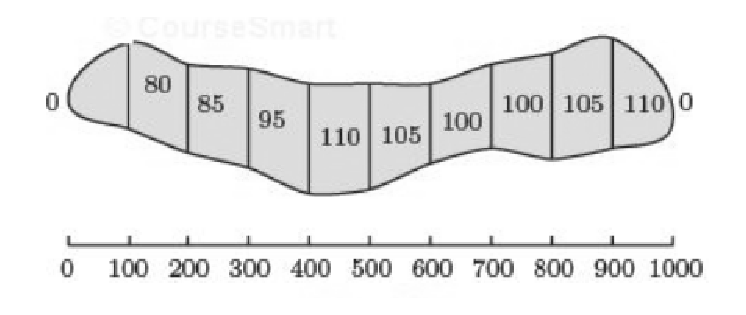
\includegraphics[width=2in]{GolfHole}
  \end{center}

~~~

\begin{Solution}
  {\bf NOTE: } In this problem, because we are only given data and not
  a function, we can only use LHR, Trapezoidal or Simpson's rules. We
  cannot use ``quad'', the adaptive integrator, because it would try
  to evaluate the function (width of the pool) in between the measured
  data points, and we don't have that information.

  Since Simpson's rule generally gives the most accurate integral
  estimate, compared with the LHR and Trapezoidal rule, we should use
  it here.

  A simple vector-based version of Simpson's rule is shown below,
  applied to these pool dimensions.


\lstinputlisting[showstringspaces=false]{MATLAB/W06Golf.m}

This script produces the estimate

``Surface area of pool is approximately 84.267 m$^2$''

This is reasonable, as the median width is 5.6 m, and the total length
of the pool is 16 m, giving approximately 89.6 m$^2$ if it were
rectangular.  This is safely in the same ballpark as the more accurate
result above.  Without more information, though, we can't improve our
integral estimate.

\end{Solution}




\item A steel scribing tip is designed to have a circular
  cross-section. The shape can be generated by rotating the function
  $\displaystyle y = \frac{0.0007}{10 x + 0.1}$ around the $x$ axis, starting at
  $x=0$ and ending at $x=0.02$ (all dimensions in meters).  Compute
  the volume of steel required to make the scribing tip.  Use an
  appropriate integration technique and parameters, and report your
  answer to five significant digits.  Be prepared to defend your
  choice of technique.

  You will need to review the volume of rotation to answer this
  question.

\begin{Solution}

  Volumes of revolution can be computed by taking slices through the
  shape.  Each slice has a volume $(\Delta x) \cdot \pi y^2$.  Adding
  up the slices using an integral gives the total volume.

  For this shape, the volume will be given by the integral
  
  $$\int_0^{0.02} \pi \left(\frac{0.0007}{10 x + 0.1}\right)^2 ~dx$$

  The analytic value of this integral is approximately $1.0262536
  \times 10^{-6}$.

  The script ``q\_3Dshape.m'' computes this integral. In the solution,
  the I used ``quad'', the adaptive integrator.  The rationale for
  this was, knowing that the integral had a value of approximately
  $10^{-6}$, I could set the absolute tolerance to $10^{-12}$, to give
  6 figures of accuracy.  Note that the ``quad'' error is only an
  estimate of the true error; however, it is usually correct within an
  order of magnitude (e.g. setting the tolerance to $10^{-12}$ usually
  ensures that the exact error is no worse that $10^{-11}$.

\end{Solution}


\item When a pendulum oscillates, with maximum deviation angle
  $\theta_0$, the period of the pendulum is given by

\begin{align*}
  T = 4 \sqrt{L/g} \int_0^{\pi/2} \frac{dx}{\sqrt{1 - k^2 \sin^2 x}}
\end{align*}

where $k = \sin\left(\frac{1}{2} \theta_0\right)$ and $g$ is the
acceleration due to gravity, $9.8 $ m/s.

Compute and compare the period of a pendulum with 
\begin{itemize}
\item $L = 2$, $\theta_0 = 40^o$, 
\item $L =2$, $\theta_0 = 20^o$.
\item $L = 2.5$, $\theta_0 = 40^o$, 
\item $L =2.5$, $\theta_0 = 20^o$.
\end{itemize}

Describe how significant the effect of maximum swing angle $\theta_0$
is on the period of a pendulum, compared to the effect of the pendulum
length.

%For fun, you can compare the period computed in this way with the
%graph of the simulated pendulum motion using differential equations
%last week.  They (should and do) agree quite closely!

\begin{Solution} 
 Full solution is available in \verb#q_pendulumPeriod.m#.

  The periods computed are show below.  ``quad'' was used for the
  integration.

L = 2.0 m, theta0 = 40.0 deg, period = 2.9274 s. \\
L = 2.0 m, theta0 = 20.0 deg, period = 2.8602 s. \\
L = 2.5 m, theta0 = 40.0 deg, period = 3.2729 s. \\
L = 2.5 m, theta0 = 20.0 deg, period = 3.1978 s. \\

From these results, it is clear that the angle has a minimal effect on
the period of the oscillations, compared with the effect of the
length.  This insensitivity of the period to the oscillation angle
explains why pendulum clocks and metronomes do not need a specific
swing angle to be fairly accurate, but {\em do} need a specific
length.
\end{Solution} 


%*******************************
\item
\begin{Question}
    
\end{Question}

\begin{Solution}
    
\end{Solution}
% Chapter Contents

% 1. Applications of the Indefinite Integral shows how to find displacement (from velocity) and velocity (from acceleration) using the indefinite integral. There are also some electronics applications in this section.

% In primary school, we learned how to find areas of shapes with straight sides (e.g. area of a triangle or rectangle). But how do you find areas when the sides are curved? We'll find out how in:

%     2. Area Under a Curve and
%     3. Area Between 2 Curves

% wine barrel

% 4. Volume of Solid of Revolution explains how to use integration to find the volume of an object with curved sides, e.g. wine barrels.

% 5. Centroid of an Area means the centre of mass. We see how to use integration to find the centroid of an area with curved sides.

% 6. Moments of Inertia explains how to find the resistance of a rotating body. We use integration when the shape has curved sides.

% 7. Work by a Variable Force shows how to find the work done on an object when the force is not constant. This section includes Hooke's Law for springs.
% Survival Tips

% Before you start this section, it's a good idea to revise:

%     Graph of the Quadratic Function
%     Graphs of Exponential and Log Functions
%     Plane Analytic Geometry
%     Curve Sketching

% (This chapter is easier if you can draw curves confidently.)

% You may also wish to see the Introduction to Calculus.

% 8. Electric Charges have a force between them that varies depending on the amount of charge and the distance between the charges. We use integration to calculate the work done when charges are separated.

% 9. Average Value of a curve can be calculated using integration.

% Head Injury Criterion is an application of average value and used in road safety research.

% 10. Force by Liquid Pressure varies depending on the shape of the object and its depth. We use integration to find the force. 

% arc length
% \hrulefill

%*******************************
\item
\begin{Question}
    
\end{Question}

\begin{Solution}
    
\end{Solution}

\end{enumerate}
\end{document}

